\documentclass[12pt]{article}

\usepackage{booktabs}
\usepackage[utf8]{inputenc}
\usepackage{amsmath, amssymb, amsthm}
\usepackage{geometry}
\usepackage{natbib}
\usepackage{setspace}
\usepackage{tikz}
\usetikzlibrary{positioning}
\usepackage{subcaption}
\usepackage{graphicx}
\usepackage{enumitem}
\usepackage{hyperref}
\usepackage{longtable}
\usepackage{booktabs}
\usepackage{bbm}
\usepackage{tikz-cd}
\usepackage{soul}
\sethlcolor{yellow} % Sets the highlight color
\usetikzlibrary{arrows.meta, positioning}
\usetikzlibrary{arrows.meta,calc,decorations.pathreplacing}

% -------------------------------------------------
% Color + framed boxes
% -------------------------------------------------
\usepackage{xcolor}
\definecolor{mygreen}{RGB}{0,140,0}
\definecolor{myblue}{RGB}{0,80,180}
\definecolor{myred}{RGB}{180,0,0}

\setlength{\fboxsep}{8pt}
\setlength{\fboxrule}{1.2pt}

\newcommand{\redbox}[1]{%
  \noindent\begingroup
  \setlength{\fboxsep}{8pt}%
  \setlength{\fboxrule}{1.2pt}%
  \fcolorbox{myred}{white}{%
    \parbox{\dimexpr\textwidth-2\fboxsep-2\fboxrule\relax}{\color{black}#1}%
  }%
  \endgroup
}

\newcommand{\bluebox}[1]{%
  \noindent\begingroup
  \setlength{\fboxsep}{8pt}%
  \setlength{\fboxrule}{1.2pt}%
  \fcolorbox{myblue}{white}{%
    \parbox{\dimexpr\textwidth-2\fboxsep-2\fboxrule\relax}{\color{black}#1}%
  }%
  \endgroup
}

\geometry{margin=1in}
\setstretch{1.5}

\DeclareMathOperator{\Var}{Var}

\newtheorem{assumption}{Assumption}
\newtheorem{lemma}{Lemma}
\theoremstyle{remark}
\newtheorem{remark}{Remark}
\newtheorem{example}{Example}
\theoremstyle{definition}
\newtheorem{corollary}{Corollary}
\newtheorem{definition}{Definition}
\newcommand{\E}{\mathbb{E}}

\def\EE{\mathbb{E}}
\def\PP{\mathbb{P}}
\def\RR{\mathbb{R}}

\title{}

\begin{document}
\maketitle

\subsection*{Subspaces}
\hfill \break  $~\!\!$ \dotfill \medskip \\

\redbox{
\textbf{Subspace Test.} Let $W \subseteq V$ where $V$ is a vector space over a field $\mathbb{F}$.

Then $W$ is a subspace of $V$ if and only if:
\begin{align*}
\forall x,y \in W,\; x+y \in W, \\
\forall a \in \mathbb{F},\; \forall x \in W,\; ax \in W.
\end{align*}
}

\medskip

\bluebox{
\textbf{Commentary:} These two conditions automatically imply:
\begin{itemize}[leftmargin=1.5em]
    \item $0 \in W$ (take $a=0$),
    \item closure under subtraction,
    \item all vector space axioms inherited from $V$.
\end{itemize}

So this is the minimal test for checking subspaces in practice.
}

\medskip
\hrule
\medskip

\subsection*{Linear Transformations}
\hfill \break  $~\!\!$ \dotfill \medskip \\

\redbox{
A map $T : V \to W$ (vector spaces over $\mathbb{F}$) is \textbf{linear} if:
\begin{align*}
T(x+y) &= T(x) + T(y), \\
T(ax) &= aT(x).
\end{align*}
}

\medskip

\bluebox{
\textbf{Commentary:} Linear maps preserve the vector space structure. In particular:
\[
T(0)=0,\quad T(x-y)=T(x)-T(y).
\]
Also, the image $T(V)$ is always a subspace of $W$.
}

\medskip
\hrule
\medskip

\subsection*{Bases and Coordinate Representation}
\hfill \break  $~\!\!$ \dotfill \medskip \\

\redbox{
Let $B=\{x_1,\dots,x_n\}$ be a basis of $V$. Then:

\begin{enumerate}[leftmargin=1.5em]
    \item $\text{span}\{x_1,\dots,x_n\}=V$
    \item $\{x_1,\dots,x_n\}$ is linearly independent
\end{enumerate}

Equivalently, every $x \in V$ can be written uniquely as
\begin{align*}
x = a_1 x_1 + \cdots + a_n x_n.
\end{align*}
}

\medskip

\bluebox{
\textbf{Commentary:} The key word is \textbf{uniquely}.

This allows us to define coordinates (coefficients of $x$ in the basis $B$):
\[
[x]_B = (a_1,\dots,a_n) \in \mathbb{F}^n.
\]

Thus choosing a basis turns an abstract vector space into $\mathbb{F}^n$.
}

\medskip
\hrule
\medskip

\subsection*{Coordinate Isomorphism}
\hfill \break  $~\!\!$ \dotfill \medskip \\

\redbox{
Define
\begin{align*}
[\cdot]_B : V \to \mathbb{F}^n, \quad x \mapsto [x]_B.
\end{align*}

Then this map is a linear isomorphism.
}

\medskip

\bluebox{
\textbf{Commentary:}
\begin{itemize}[leftmargin=1.5em]
    \item Linearity follows from linearity of coordinates:
    \[
    [x+y]_B = [x]_B + [y]_B,\quad [ax]_B = a[x]_B.
    \]
    \item Injective: unique representation
    \item Surjective: every vector in $\mathbb{F}^n$ corresponds to some $x$
\end{itemize}

So all finite-dimensional vector spaces of dimension $n$ are essentially $\mathbb{F}^n$.
}

\medskip
\hrule
\medskip

\subsection*{Matrix Representation of a Linear Map}
\hfill \break  $~\!\!$ \dotfill \medskip \\

\redbox{
Let $T: V \to W$ be linear, with bases $B$ for $V$ and $C$ for $W$.

Then there exists a matrix $[T]_{C \leftarrow B}$ such that
\begin{align*}
[T(x)]_C = [T]_{C \leftarrow B} \,[x]_B.
\end{align*}
}

\medskip

\bluebox{
\textbf{Commentary:}
\begin{itemize}[leftmargin=1.5em]
    \item The matrix is constructed by applying $T$ to basis vectors:
    \[
    [T(x_j)]_C = \text{column } j.
    \]
    \item This converts abstract linear maps into matrix multiplication.
\end{itemize}

So linear algebra = matrix algebra once a basis is fixed.
}

\medskip
\hrule
\medskip

\subsection*{Change of Basis}
\hfill \break  $~\!\!$ \dotfill \medskip \\

\redbox{
Let $B,B'$ be two bases of $V$. Then there exists an invertible matrix $Q$ such that
\begin{align*}
[x]_{B'} = Q [x]_B.
\end{align*}

$Q$ is called the \textbf{change of coordinate matrix} from $B$ to $B'$.
}

\medskip

\bluebox{
\textbf{Commentary:}
\begin{itemize}[leftmargin=1.5em]
    \item Columns of $Q$ are the coordinates of the new basis vectors in the old basis.
    \item $Q$ is always invertible.
    \item $Q^{-1}$ converts back.
\end{itemize}

So coordinates depend on basis, but the underlying vector does not.
}

\medskip
\hrule
\medskip

\subsection*{Change of Matrix Representation}
\hfill \break  $~\!\!$ \dotfill \medskip \\

\redbox{
Let $T: V \to V$ and let $B,B'$ be two bases.

If $Q$ is the change-of-basis matrix, then
\begin{align*}
[T]_{B'} = Q [T]_B Q^{-1}.
\end{align*}
}

\medskip

\bluebox{
\textbf{Commentary:}
This is called a \textbf{similarity transformation}.

It shows:
\begin{itemize}[leftmargin=1.5em]
    \item Different matrices can represent the same linear operator
    \item They are related by conjugation
    \item $T$ is the actual linear transformation between vector spaces.
    \item $[T]_B$ is the matrix that represents $T$ once basis $B$ is chosen.
\end{itemize}

This is the foundation of:
\begin{itemize}[leftmargin=1.5em]
    \item diagonalization
    \item eigenvalues
    \item canonical forms
\end{itemize}
}

\medskip
\hrule
\medskip

\subsection*{Big Picture Diagram}
\hfill \break  $~\!\!$ \dotfill \medskip \\

\bluebox{
\textbf{Conceptual Summary:}

\[
\begin{array}{ccc}
V & \xrightarrow{T} & V \\
\downarrow [\cdot]_B & & \downarrow [\cdot]_B \\
\mathbb{F}^n & \xrightarrow{[T]_B} & \mathbb{F}^n
\end{array}
\]

Changing basis inserts $Q$:

\[
[T]_{B'} = Q [T]_B Q^{-1}.
\]

So:
\begin{itemize}[leftmargin=1.5em]
    \item Abstract map $\leftrightarrow$ matrix
    \item Basis choice $\leftrightarrow$ coordinate system
    \item Change of basis $\leftrightarrow$ similarity transform
\end{itemize}
}

\bluebox{
$V$ and $\mathbb{F}^n$ are usually \textbf{isomorphic}, not \textbf{equal}.

When we say $V$ is an $n$-dimensional vector space over $F$, that means $V$ has the same vector-space structure as $F^n$, but its elements need not already be $n$-tuples.

So the distinction is: $V \cong F^n$ but usually not $V = F^n$. 

A vector space is not determined just by ``field $F$ + dimension $n$'' as a set. Many different-looking objects can all be $n$-dimensional vector spaces over $F$.

Examples of $2$-dimensional vector spaces over $\mathbb{R}$:

- $\mathbb{R}^2$
- the space of polynomials of degree $\le 1$, $P_1(\mathbb{R})$
- the space of $2\times 2$ diagonal matrices
- any plane through the origin in $\mathbb{R}^3$

All of these are $2$-dimensional over $\mathbb{R}$, so each is isomorphic to $\mathbb{R}^2$, but they are not the same set and their elements do not look the same.
}

\bluebox{
For instance, in $P_1(\mathbb{R})$, a vector looks like $a+bx$, not like $(a,b)$.

Once you choose an ordered basis, say $B=(1,x)$, then every polynomial $a+bx$ gets identified with its coordinate vector $[a+bx]_B=\begin{pmatrix} a \\ b \end{pmatrix}\in\mathbb{R}^2$.

That coordinate map is the isomorphism.

So the reason I distinguish $V$ and $F^n$ is:

- $V$ is the original abstract vector space
- $F^n$ is the coordinate model you get after choosing a basis

A basis gives a specific map $[\cdot]_B:V\to F^n$, and that map depends on the basis.

Without choosing a basis, there is no canonical way to say which vector in $V$ corresponds to which tuple in $F^n$.

That is why $V$ is not automatically $F^n$. It becomes identified with $F^n$ only after a basis is chosen.

A useful analogy: two sets can have the same number of elements without being literally the same set. Likewise, two vector spaces can have the same dimension over the same field without being literally the same vector space.

So the clean statement is:

\textbf{Every $n$-dimensional vector space over $F$ is isomorphic to $\mathbb{F}^n$, but not automatically equal to $F^n$.}

The only time you would write $V=F^n$ is when the vector space actually has already been defined to be $F^n$.
}

\subsection*{Vector Spaces and Subspaces}

Let $F$ be a field and let $V$ be a vector space over $F$.

A subset $W \subseteq V$ is called a \emph{subspace} if:
\begin{enumerate}
    \item $0 \in W$,
    \item $x,y \in W \Rightarrow x+y \in W$,
    \item $a \in F,\, x \in W \Rightarrow ax \in W$.
\end{enumerate}

\begin{center}
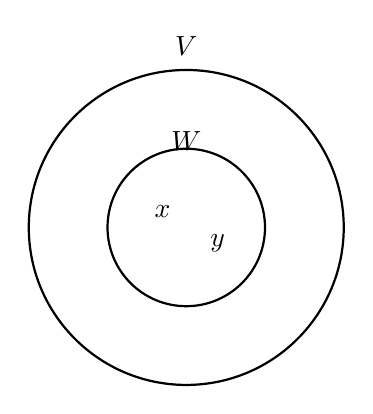
\begin{tikzpicture}
  \draw[thick] (0,0) circle (2);
  \draw[thick] (0,0) circle (1);
  \node at (0,2.3) {$V$};
  \node at (0,1.1) {$W$};
  \node at (-0.3,0.2) {$x$};
  \node at (0.4,-0.2) {$y$};
\end{tikzpicture}
\end{center}

\subsection*{Linear Transformations}

Let $V,W$ be vector spaces over $F$.
A function $T: V \to W$ is called a \emph{linear transformation} if
\[
T(x+y) = T(x) + T(y), \qquad T(ax) = aT(x)
\]
for all $x,y \in V$ and $a \in F$.

\subsection*{Bases and Coordinates}

Let $V$ be an $n$--dimensional vector space over $F$.
An ordered set
\[
\mathcal{B} = \{x_1,\dots,x_n\}
\]
is a \emph{basis} of $V$ if:
\begin{enumerate}
    \item $\operatorname{span}\{x_1,\dots,x_n\} = V$,
    \item $\{x_1,\dots,x_n\}$ is linearly independent.
\end{enumerate}

Every $x \in V$ can be written uniquely as

\[
x = a_1 x_1 + \cdots + a_n x_n,
\qquad a_i \in F.
\]

Define the coordinate vector of $x$ relative to $\mathcal{B}$ by

\[
[x]_{\mathcal{B}} =
\begin{bmatrix}
a_1 \\ \vdots \\ a_n
\end{bmatrix}
\in F^n.
\]

\subsection*{Coordinate Map Is an Isomorphism}

Define the map
\[
\Phi_{\mathcal{B}} : V \to F^n,
\qquad
\Phi_{\mathcal{B}}(x) = [x]_{\mathcal{B}}.
\]

Then $\Phi_{\mathcal{B}}$ is a linear isomorphism.

\begin{center}
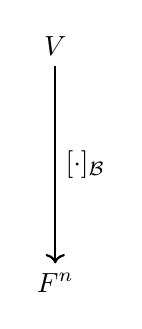
\begin{tikzpicture}[node distance=3cm]
\node (V) {$V$};
\node (Fn) [below of=V] {$F^n$};

\draw[->, thick] (V) -- node[right] {$[\cdot]_{\mathcal{B}}$} (Fn);
\end{tikzpicture}
\end{center}

Let $\mathcal{B}$ and $\mathcal{B}'$ be two ordered bases of $V$. Note that order matters because coordinates depend on it.



\subsection*{Change of Basis Matrix}

There exists an invertible matrix $Q \in F^{n \times n}$ such that
\[
[x]_{\mathcal{B}} = Q [x]_{\mathcal{B}'}.
\]

The matrix $Q$ is called the \emph{change of coordinate matrix}
from $\mathcal{B}'$ to $\mathcal{B}$.

\begin{center}
\begin{tikzcd}
V \arrow[d, "{[\cdot]_{\mathcal{B}'}}"'] \arrow[dr, "{[\cdot]_{\mathcal{B}}}"] & \\
F^n \arrow[r, "Q"] & F^n
\end{tikzcd}
\end{center}

\subsection*{Matrix Representation of Linear Transformations}

Let $T: V \to V$ be linear and let $\mathcal{B}$ be a basis of $V$.

There exists a unique matrix $[T]_{\mathcal{B}} \in F^{n \times n}$ such that
\[
[T(x)]_{\mathcal{B}} = [T]_{\mathcal{B}} [x]_{\mathcal{B}}
\]
for all $x \in V$.

\begin{center}
\begin{tikzcd}[column sep=huge, row sep=huge]
V \arrow[r, "T"]
  \arrow[d, shift right=2pt, "{[\cdot]_{\mathcal{B}'}}"']
& V \arrow[d, shift left=2pt, "{[\cdot]_{\mathcal{B}'}}"] \\
F^n \arrow[r, "{[T]_{\mathcal{B}'}}"]
    \arrow[u, shift right=2pt, "Q"']
& F^n \arrow[u, shift left=2pt, "Q"]
\end{tikzcd}
\end{center}

The key insight the diagram captures is that the square commutes — there are two paths from $V$ (top-left) to $\mathbb{F}^n$ (bottom-right), and they always give the same answer. 

\textbf{Route 1:} Apply $T$ first (stay in abstract $V$), then coordinatize via $[\cdot]_{\mathcal{B}}$.

\textbf{Route 2:} Coordinatize $x$ first to get $[x]_{\mathcal{B}} \in F^n$, then multiply by the matrix $[T]_{\mathcal{B}}$.

The theorem says these are identical, which is exactly what $    [T(x)]_{\mathcal{B}} = [T]_{\mathcal{B}}\, [x]_{\mathcal{B}}$ asserts. The matrix $[T]_{\mathcal{B}}$ exists precisely to make this square commute---it translates the abstract linear map $T$ into concrete matrix multiplication in coordinate space $F^n$.

Let $\mathcal{B}, \mathcal{B}'$ be two bases and let $Q$ be the change-of-basis matrix.


\subsection*{Change of Basis and Similar Matrices}

Let $T : V \to V$ be a linear map, and let $\mathcal{B}$ and $\mathcal{B}'$ be two bases of $V$.
Let $Q$ be the change-of-basis matrix from $\mathcal{B}'$ to $\mathcal{B}$, so that
$[x]_{\mathcal{B}} = Q\,[x]_{\mathcal{B}'}$ for all $x \in V$.

\medskip
The matrix representations of $T$ in the two bases satisfy
\[
    [T]_{\mathcal{B}} \;=\; Q\,[T]_{\mathcal{B}'}\,Q^{-1}.
\]
Thus, different matrix representations of the same linear operator are \emph{similar matrices}.

\medskip
\noindent\textbf{Commutative diagram.}
The identity is witnessed by the following commutative square,
in which both routes from $V$ (top-left) to $F^n$ (bottom-right) agree.

Original diagram from lecture:\\

\begin{center}
\begin{tikzcd}[column sep=8em, row sep=6em]
F^n \arrow[r, "{[T]_{\mathcal{B}'}}"] 
    \arrow[d, shift right=2ex, "Q"'] 
& F^n \arrow[d, shift left=2ex, "Q"] \\
F^n \arrow[r, "{[T]_{\mathcal{B}}}"] 
    \arrow[u, shift right=2ex, "Q^{-1}"] 
& F^n \arrow[u, shift left=2ex, "Q^{-1}"']
\end{tikzcd}
\end{center}



\noindent The key insight is that the diagram is \emph{not} showing two
separate maps per side. Rather, it is showing one isomorphism per side
with both the forward and backward directions labeled simultaneously.
Specifical

More detailed version:\\
\begin{center}
\begin{tikzcd}[column sep=huge, row sep=large]
V \arrow[r, "T"] \arrow[d, "{[\cdot]_{\mathcal{B}'}}"']
& V \arrow[d, "{[\cdot]_{\mathcal{B}'}}"] \\
F^n \arrow[r, "{[T]_{\mathcal{B}'}}"] \arrow[d, "Q"']
& F^n \arrow[d, "Q"] \\
F^n \arrow[r, "{[T]_{\mathcal{B}}}"] \arrow[u, bend right=40, "Q^{-1}"']
& F^n
\end{tikzcd}
\end{center}

\medskip
\noindent\textbf{Step-by-step verification.}
Fix $x \in V$.

\begin{enumerate}
    \item \textbf{Route 1 (top, then right):}
    Apply $T$ to get $T(x) \in V$, then coordinatize in $\mathcal{B}'$:
    \[
        x \;\xrightarrow{\;T\;}\; T(x)
          \;\xrightarrow{\;[\cdot]_{\mathcal{B}'}\;}\;
          [T(x)]_{\mathcal{B}'} \;=\; [T]_{\mathcal{B}'}\,[x]_{\mathcal{B}'}
          \;\in\; F^n.
    \]

    \item \textbf{Route 2 (left, then bottom):}
    Convert $x$ from $\mathcal{B}$-coordinates to $\mathcal{B}'$-coordinates via $Q^{-1}$,
    then apply $[T]_{\mathcal{B}'}$:
    \[
        x \;\xrightarrow{\;Q^{-1} \circ [\cdot]_{\mathcal{B}}\;}\;
          Q^{-1}[x]_{\mathcal{B}} \;=\; [x]_{\mathcal{B}'}
          \;\xrightarrow{\;[T]_{\mathcal{B}'}\;}\;
          [T]_{\mathcal{B}'}\,Q^{-1}[x]_{\mathcal{B}}
          \;\in\; F^n.
    \]

    \item \textbf{Commutativity:}
    Both routes produce the same element of $F^n$, so for all $x \in V$:
    \[
        [T]_{\mathcal{B}'}\,[x]_{\mathcal{B}'} \;=\; [T]_{\mathcal{B}'}\,Q^{-1}[x]_{\mathcal{B}}.
    \]
    Since $[x]_{\mathcal{B}'} = Q^{-1}[x]_{\mathcal{B}}$, this is consistent.
    Now recall that by definition of $[T]_{\mathcal{B}}$:
    \[
        [T(x)]_{\mathcal{B}} \;=\; [T]_{\mathcal{B}}\,[x]_{\mathcal{B}}.
    \]
    Expressing $[T(x)]_{\mathcal{B}} = Q\,[T(x)]_{\mathcal{B}'}
    = Q\,[T]_{\mathcal{B}'}\,Q^{-1}[x]_{\mathcal{B}}$
    and equating with $[T]_{\mathcal{B}}\,[x]_{\mathcal{B}}$ gives,
    since this holds for all $x$:
    \[
        \boxed{[T]_{\mathcal{B}} \;=\; Q\,[T]_{\mathcal{B}'}\,Q^{-1}.}
    \]

    \item \textbf{Geometric reading of $Q\,[T]_{\mathcal{B}'}\,Q^{-1}$:}
    Reading right to left, $Q^{-1}$ converts input coordinates from $\mathcal{B}$
    to $\mathcal{B}'$ (left arrow, going down); $[T]_{\mathcal{B}'}$ applies the
    transformation in the $\mathcal{B}'$-coordinate system (bottom arrow, going right);
    and $Q$ converts the result back from $\mathcal{B}'$-coordinates to
    $\mathcal{B}$-coordinates. The conjugation $Q\,(\cdot)\,Q^{-1}$ is a round-trip
    change of coordinates sandwiching the computation.
\end{enumerate}

\noindent\textbf{Where does $[x]_{\mathcal{B}'}$ come from?}

\medskip
The change-of-basis matrix $Q$ is defined by the relation
\[
    [x]_{\mathcal{B}} \;=\; Q\,[x]_{\mathcal{B}'}
    \qquad \text{for all } x \in V.
\]
Multiplying both sides on the left by $Q^{-1}$ gives immediately
\[
    Q^{-1}[x]_{\mathcal{B}} \;=\; [x]_{\mathcal{B}'}.
\]
This is the entire justification---no separate computation is needed.

\medskip
The left vertical arrow in the commutative diagram is labeled
$Q^{-1} \circ [\cdot]_{\mathcal{B}}$, which decomposes into two steps:
\begin{enumerate}
    \item Apply $[\cdot]_{\mathcal{B}}$: extract the $\mathcal{B}$-coordinates
    of $x$, producing $[x]_{\mathcal{B}} \in F^n$.
    \item Multiply by $Q^{-1}$: convert from $\mathcal{B}$-coordinates to
    $\mathcal{B}'$-coordinates, producing $Q^{-1}[x]_{\mathcal{B}} = [x]_{\mathcal{B}'} \in F^n$.
\end{enumerate}
The composition $Q^{-1} \circ [\cdot]_{\mathcal{B}}$ therefore sends $x \mapsto [x]_{\mathcal{B}'}$,
which is exactly the coordinatization map $[\cdot]_{\mathcal{B}'}$ applied directly.


\noindent\textbf{Reconciliation with the original diagram.}

The vertical arrows in the diagram are isomorphisms, and the diagram
labels both directions simultaneously. Specifically, the
coordinatization map $[\cdot]_{\mathcal{B}'} : V \to F^n$ is an
isomorphism whose inverse is $Q : F^n \to V$, since $Q$ reconstructs
an abstract vector from its $\mathcal{B}'$-coordinates:
\[
    Q\,[x]_{\mathcal{B}'} \;=\; x
    \qquad \Longleftrightarrow \qquad
    [\cdot]_{\mathcal{B}'} \;=\; Q^{-1}.
\]
Thus on each vertical side, the two labels refer to the \emph{same}
isomorphism viewed in opposite directions:
\begin{itemize}
    \item Left side going down: $[\cdot]_{\mathcal{B}'} = Q^{-1}$
    \item Left side going up: $Q^{-1}$ --- same map, inverse direction shown for clarity
    \item Right side going down: $[\cdot]_{\mathcal{B}'} = Q^{-1}$
    \item Right side going up: $Q$ --- the inverse, reconstructing $x \in V$
\end{itemize}
The commutative square then reads: starting from $x \in V$ in the
top-left, both routes to $F^n$ in the bottom-right agree:
\begin{align*}
\text{Route 1 (top then right):} &\quad
    x \xrightarrow{T} T(x) \xrightarrow{[\cdot]_{\mathcal{B}'}} [T(x)]_{\mathcal{B}'} \\
\text{Route 2 (left then bottom):} &\quad
    x \xrightarrow{Q^{-1}} [x]_{\mathcal{B}'} \xrightarrow{[T]_{\mathcal{B}'}} [T]_{\mathcal{B}'}[x]_{\mathcal{B}'}
\end{align*}
Commutativity gives $[T(x)]_{\mathcal{B}'} = [T]_{\mathcal{B}'}[x]_{\mathcal{B}'}$
for all $x \in V$, which is precisely the definition of $[T]_{\mathcal{B}'}$.
The relation $[T]_{\mathcal{B}} = Q[T]_{\mathcal{B}'}Q^{-1}$ then follows
by conjugating both sides by $Q$.


\subsection*{Vector Spaces and Subspaces}
\hfill \break  $~\!\!$ \dotfill \medskip \\

\redbox{
\textbf{Subspace Test.} Let $W \subseteq V$ where $V$ is a vector space over $\mathbb{F}$.

Then $W$ is a subspace iff:
\begin{align*}
\text{(i)}\; x,y \in W \Rightarrow x+y \in W, \\
\text{(ii)}\; a \in \mathbb{F}, x \in W \Rightarrow ax \in W.
\end{align*}
}

\medskip

\bluebox{
This implies automatically:
\[
0 \in W,\quad x-y \in W.
\]
So closure under addition + scalar multiplication is sufficient.
}

\medskip
\hrule
\medskip

\subsection*{Sum and Direct Sum of Subspaces}

\redbox{
Let $W_1, W_2 \subseteq V$ be subspaces.

\[
W_1 + W_2 = \{x_1 + x_2 : x_1 \in W_1, x_2 \in W_2\}.
\]

Then $W_1 + W_2$ is a subspace and is the smallest subspace containing both.
}

\medskip

\bluebox{
Union $W_1 \cup W_2$ is generally NOT a subspace (fails closure).
Sum fixes this by enforcing closure.
}

\medskip
\hrule
\medskip

\redbox{
\textbf{Direct Sum.}
\[
V = W_1 \oplus W_2
\]
iff every $v \in V$ can be written uniquely as
\[
v = x_1 + x_2,\quad x_1 \in W_1,\; x_2 \in W_2.
\]
}

\medskip

\bluebox{
Equivalent condition:
\[
W_1 \cap W_2 = \{0\}.
\]

Uniqueness proof (missing in notes):

If
\[
x_1 + x_2 = y_1 + y_2,
\]
then
\[
x_1 - y_1 = y_2 - x_2 \in W_1 \cap W_2,
\]
so both sides are $0$, hence uniqueness.
}

\medskip
\hrule
\medskip

\subsection*{Basis and Coordinates}

\redbox{
A set $B=\{x_1,\dots,x_n\}$ is a basis of $V$ iff:
\begin{align*}
\text{(i)}\; \text{span}(B)=V, \\
\text{(ii)}\; B \text{ is linearly independent}.
\end{align*}

Then every $x \in V$ can be written uniquely:
\[
x = a_1 x_1 + \cdots + a_n x_n.
\]
}

\medskip

\bluebox{
Define coordinate map:
\[
[x]_B = (a_1,\dots,a_n) \in \mathbb{F}^n.
\]

This gives an isomorphism:
\[
V \cong \mathbb{F}^n.
\]
}

\medskip
\hrule
\medskip

\subsection*{Linear Maps}

\redbox{
A map $T:V \to W$ is linear iff:
\[
T(x+y)=T(x)+T(y),\quad T(ax)=aT(x).
\]
}

\medskip

\bluebox{
Then:
\[
T(0)=0,\quad T(\text{span}) = \text{span}.
\]

Also $\text{Im}(T)$ is a subspace.
}

\medskip
\hrule
\medskip

\subsection*{Matrix Representation}

\redbox{
Given bases $B,C$, there exists a matrix $[T]_{C \leftarrow B}$ such that:
\[
[T(x)]_C = [T]_{C \leftarrow B}[x]_B.
\]
}

\medskip

\bluebox{
Columns = images of basis vectors.

This converts linear maps into matrix multiplication.
}

\medskip
\hrule
\medskip

\subsection*{Change of Basis}

\redbox{
If $B,B'$ are bases, then:
\[
[x]_{B'} = Q [x]_B,
\]
where $Q$ is invertible.
}

\medskip

\redbox{
\[
[T]_{B'} = Q [T]_B Q^{-1}.
\]
}

\medskip

\bluebox{
This is similarity transformation $\to$ same operator, different matrix.
}

\medskip
\hrule
\medskip

\subsection*{Inner Product Spaces}

\redbox{
An inner product $\langle \cdot,\cdot\rangle$ satisfies:
\begin{align*}
\langle v,v\rangle \ge 0,\quad \langle v,v\rangle=0 \iff v=0,\\
\langle u,v\rangle = \overline{\langle v,u\rangle},\\
\langle ru+sw, v\rangle = r\langle u,v\rangle + s\langle w,v\rangle.
\end{align*}
}

\medskip
\hrule
\medskip

\subsection*{Norms}

\redbox{
A norm $\|\cdot\|$ satisfies:
\begin{align*}
\|u\|\ge 0,\quad \|u\|=0 \iff u=0,\\
\|\alpha u\|=|\alpha|\|u\|,\\
\|u+v\|\le \|u\|+\|v\|.
\end{align*}
}

\medskip

\bluebox{
From inner product:
\[
\|u\| = \sqrt{\langle u,u\rangle}.
\]
}

\medskip
\hrule
\medskip

\subsection*{Cauchy--Schwarz Inequality}

\redbox{
\[
|\langle u,v\rangle| \le \|u\|\|v\|.
\]
}

\medskip

\bluebox{
Proof idea (filled):

Consider:
\[
\|u - \lambda v\|^2 \ge 0,
\]
choose $\lambda = \frac{\langle u,v\rangle}{\langle v,v\rangle}$.
}

\medskip
\hrule
\medskip

\subsection*{Triangle Inequality}

\redbox{
\[
\|u+v\| \le \|u\| + \|v\|.
\]
}

\medskip

\bluebox{
Use:
\[
\|u+v\|^2 = \|u\|^2 + \|v\|^2 + 2\text{Re}\langle u,v\rangle
\]
then apply Cauchy--Schwarz.
}

\medskip
\hrule
\medskip

\subsection*{Metric Spaces}

\redbox{
A metric $d$ satisfies:
\begin{align*}
d(x,y)\ge0,\quad d(x,y)=0 \iff x=y,\\
d(x,y)=d(y,x),\\
d(x,z)\le d(x,y)+d(y,z).
\end{align*}
}

\medskip

\redbox{
From norm:
\[
d(x,y)=\|x-y\|
\]
is a metric.
}

\medskip
\hrule
\medskip

\subsection*{Banach and Hilbert Spaces}

\redbox{
A normed space is \textbf{Banach} if complete.

An inner product space is \textbf{Hilbert} if complete under induced norm.
}

\medskip
\hrule
\medskip

\subsection*{Parallelogram Law}

\redbox{
\[
\|x+y\|^2 + \|x-y\|^2 = 2(\|x\|^2 + \|y\|^2).
\]
}

\medskip

\bluebox{
Characterizes norms coming from inner products.
}

\medskip
\hrule
\medskip

\subsection*{Polarization Identity}

\redbox{
Over $\mathbb{R}$:
\[
\langle x,y\rangle = \frac{1}{4}(\|x+y\|^2 - \|x-y\|^2).
\]
}

\medskip

\redbox{
Over $\mathbb{C}$:
\[
\langle x,y\rangle = \frac{1}{4}\left(\|x+y\|^2 - \|x-y\|^2 + i\|x+iy\|^2 - i\|x-iy\|^2\right).
\]
}

\medskip
\hrule
\medskip

\subsection*{Isometries}

\redbox{
$T$ is an isometry iff:
\[
\|T(v)\| = \|v\|
\quad \Longleftrightarrow \quad
\langle T(u),T(v)\rangle = \langle u,v\rangle.
\]
}

\medskip
\hrule
\medskip

\subsection*{Bounded Linear Operators}

\redbox{
$T:X\to Y$ is bounded iff:
\[
\|T(u)\| \le M\|u\|.
\]

Operator norm:
\[
\|T\| = \sup_{\|u\|=1}\|T(u)\|.
\]
}

\medskip

\redbox{
\textbf{Theorem.} $T$ is continuous iff bounded.
}

\medskip

\bluebox{
Finite-dimensional result:

Every linear map is bounded.
}

\medskip
\hrule
\medskip

\subsection*{Space of Operators}

\redbox{
\[
\mathcal{L}(X,Y)
\]
is a vector space.
}

\medskip

\bluebox{
Dimension (finite case):
\[
\dim(\mathcal{L}(X,Y)) = \dim(X)\cdot\dim(Y).
\]
}

\subsection*{Bounded Linear Operators and Operator Norm}
\hfill \break  $~\!\!$ \dotfill \medskip \\

\textbf{Definition.}\\
\redbox{
Let $(X,\|\cdot\|_X)$ and $(Y,\|\cdot\|_Y)$ be normed vector spaces.\\

A linear operator $T : X \to Y$ is said to be \textbf{bounded} if there exists $M \ge 0$ such that
\begin{align*}
\|T(u)\|_Y \le M \|u\|_X \quad \text{for all } u \in X.
\end{align*}

The infimum of all such $M$ is called the \textbf{operator norm} of $T$, denoted by
\begin{align*}
\|T\|.
\end{align*}
}

\medskip

\bluebox{
\textbf{Commentary:} The operator norm can be written explicitly as
\begin{align*}
\|T\| = \sup_{\|u\|_X = 1} \|T(u)\|_Y.
\end{align*}
This shows that $\|T\|$ measures the maximum stretching effect of $T$ on unit vectors.
}

\medskip
\hrule
\medskip

\subsection*{Theorem 1: Continuity $\Leftrightarrow$ Boundedness}
\hfill \break  $~\!\!$ \dotfill \medskip \\

\redbox{
\textbf{Theorem.} A linear operator $T : X \to Y$ between normed vector spaces is continuous if and only if it is bounded.
}

\medskip

\textbf{Proof.}

\textbf{($\Leftarrow$)} Suppose $T$ is bounded.

\redbox{
Then there exists $M \ge 0$ such that
\begin{align*}
\|T(u)\| \le M \|u\| \quad \forall u \in X.
\end{align*}

For any $u,v \in X$,
\begin{align*}
\|T(u) - T(v)\| &= \|T(u - v)\| \\
&\le M \|u - v\|.
\end{align*}

Thus $T$ is Lipschitz, hence continuous.
}

\medskip

\bluebox{
\textbf{Commentary:} The key step is using linearity:
\[
T(u) - T(v) = T(u - v).
\]
This reduces continuity everywhere to behavior at $0$. Lipschitz continuity immediately implies continuity.
}

\medskip
\hrule
\medskip

\textbf{($\Rightarrow$)} Suppose $T$ is continuous.

\redbox{
Since $T$ is linear, $T(0)=0$.\\

Continuity at $0$ implies: for $\varepsilon = 1$, there exists $\delta > 0$ such that
\begin{align*}
\|u\| < \delta \implies \|T(u)\| < 1.
\end{align*}

Let $u \neq 0$ and define
\begin{align*}
\lambda = \frac{\delta}{\|u\|}.
\end{align*}

Then $\|\lambda u\| = \delta$, so
\begin{align*}
\|T(\lambda u)\| < 1.
\end{align*}

By linearity,
\begin{align*}
\|T(\lambda u)\| = |\lambda| \|T(u)\|.
\end{align*}

Thus,
\begin{align*}
\|T(u)\| < \frac{1}{\lambda} = \frac{\|u\|}{\delta}.
\end{align*}

Hence
\begin{align*}
\|T(u)\| \le \frac{1}{\delta} \|u\|.
\end{align*}

So $T$ is bounded.
}

\medskip

\bluebox{
\textbf{Commentary:} The trick is scaling $u$ so that it lies inside the $\delta$-ball where we control $T$. This is a standard argument showing that linear + continuity at $0$ implies global boundedness.

Also note: continuity at a single point ($0$) is enough due to linearity.
}

\medskip
\hrule
\medskip

\subsection*{Finite Dimensional Case}
\hfill \break  $~\!\!$ \dotfill \medskip \\

\redbox{
\textbf{Theorem.} If $\dim(X) < \infty$, then every linear operator $T : X \to Y$ is bounded.
}

\medskip

\bluebox{
\textbf{Commentary:} This follows because all norms on finite-dimensional spaces are equivalent, and linear maps are continuous in finite dimensions. Hence boundedness is automatic.

This is why infinite-dimensional spaces are where boundedness becomes a real condition.
}

\medskip
\hrule
\medskip

\subsection*{Vector Space of Linear Operators}
\hfill \break  $~\!\!$ \dotfill \medskip \\

\redbox{
\textbf{Claim.} If $T,S : X \to Y$ are linear operators, then for any scalars $\alpha,\beta$,
\begin{align*}
\alpha T + \beta S
\end{align*}
is also a linear operator.

Hence the collection of all linear operators from $X$ to $Y$ forms a vector space.
}

\medskip

\bluebox{
\textbf{Commentary:} This is checked directly:
\begin{align*}
(\alpha T + \beta S)(u+v) &= \alpha T(u+v) + \beta S(u+v) \\
&= \alpha(Tu + Tv) + \beta(Su + Sv),
\end{align*}
and similarly for scalar multiplication.

So linear operators are closed under addition and scalar multiplication.
}

\medskip
\hrule
\medskip

\subsection*{Theorem 2: $\mathcal{L}(X,Y)$ is a Normed Space}
\hfill \break  $~\!\!$ \dotfill \medskip \\

\redbox{
\textbf{Theorem.} Let $X,Y$ be normed vector spaces. Then the collection of bounded linear operators
\[
\mathcal{L}(X,Y)
\]
is a normed vector space with norm $\|\cdot\|$ (the operator norm).
}

\medskip

\textbf{Proof.}

\redbox{
Let $T,S \in \mathcal{L}(X,Y)$. Then for all $u \in X$,
\begin{align*}
\|(T+S)(u)\| &= \|T(u) + S(u)\| \\
&\le \|T(u)\| + \|S(u)\| \\
&\le \|T\|\|u\| + \|S\|\|u\| \\
&= (\|T\| + \|S\|)\|u\|.
\end{align*}

Thus $T+S$ is bounded and
\begin{align*}
\|T+S\| \le \|T\| + \|S\|.
\end{align*}
}

\medskip

\bluebox{
\textbf{Commentary:} This proves both:
\begin{itemize}[leftmargin=1.5em]
    \item closure under addition (boundedness preserved),
    \item triangle inequality for the operator norm.
\end{itemize}

Similarly, one can check:
\[
\|\alpha T\| = |\alpha|\|T\|
\]
and $\|T\| = 0 \iff T=0$.

Hence $\mathcal{L}(X,Y)$ is a normed vector space.
}

\subsection*{Properties of the Operator Norm}
\hfill \break  $~\!\!$ \dotfill \medskip \\

\textbf{Triangle Inequality.}

\redbox{
For $T,S \in \mathcal{L}(X,Y)$,
\begin{align*}
\|T+S\| \le \|T\| + \|S\|.
\end{align*}
}

\medskip

\bluebox{
\textbf{Commentary:} From the estimate
\[
\|(T+S)(u)\| \le (\|T\| + \|S\|)\|u\|,
\]
the inequality follows by taking the infimum over all admissible constants $M$ in the definition of the operator norm.
}

\medskip
\hrule
\medskip

\textbf{Homogeneity.}

\redbox{
For any scalar $\alpha$ and $T \in \mathcal{L}(X,Y)$,
\begin{align*}
\|\alpha T\| = |\alpha| \|T\|.
\end{align*}
}

\medskip

\redbox{
\textbf{Proof.}
\begin{align*}
\|(\alpha T)(u)\| &= |\alpha|\|T(u)\| \\
&\le |\alpha| \|T\| \|u\|.
\end{align*}
Thus $\|\alpha T\| \le |\alpha|\|T\|$.

Conversely, applying this to $\frac{1}{\alpha}(\alpha T)=T$ (for $\alpha \neq 0$),
\[
\|T\| \le \frac{1}{|\alpha|}\|\alpha T\|,
\]
so $\|\alpha T\| = |\alpha|\|T\|$.
}

\medskip

\bluebox{
\textbf{Commentary:} This shows the operator norm behaves exactly like a norm should under scalar multiplication. The reverse inequality is often omitted on the board but is essential.
}

\medskip
\hrule
\medskip

\textbf{Definiteness.}

\redbox{
\begin{align*}
\|T\| = 0 \iff T = 0.
\end{align*}
}

\medskip

\redbox{
\textbf{Proof.}

If $\|T\| = 0$, then
\[
\|T(u)\| \le 0 \cdot \|u\| = 0 \quad \forall u,
\]
so $T(u)=0$ for all $u$, hence $T=0$.

Conversely, if $T=0$, then clearly $\|T\|=0$.
}

\medskip

\bluebox{
\textbf{Commentary:} This verifies that the operator norm is a true norm (not just a seminorm).
}

\medskip
\hrule
\medskip

\subsection*{Theorem 3: Completeness of $\mathcal{L}(X,Y)$}
\hfill \break  $~\!\!$ \dotfill \medskip \\

\redbox{
\textbf{Theorem.} Let $X,Y$ be normed vector spaces. If $Y$ is Banach, then
\[
\mathcal{L}(X,Y)
\]
is a Banach space (i.e., complete under the operator norm).
}

\medskip

\textbf{Proof.}

\redbox{
Let $\{T_n\}$ be a Cauchy sequence in $\mathcal{L}(X,Y)$. Then for all $u \in X$,
\begin{align*}
\|T_n(u) - T_m(u)\| &= \|(T_n - T_m)(u)\| \\
&\le \|T_n - T_m\| \|u\|.
\end{align*}

Thus $\{T_n(u)\}$ is a Cauchy sequence in $Y$ for each fixed $u$.

Since $Y$ is Banach, there exists $T(u) \in Y$ such that
\begin{align*}
T(u) = \lim_{n\to\infty} T_n(u).
\end{align*}
}

\medskip

\bluebox{
\textbf{Commentary:} This defines a candidate limit operator pointwise. The key idea is: completeness transfers from $Y$ to the space of operators.
}

\medskip
\hrule
\medskip

\textbf{Step 1: Linearity of $T$}

\redbox{
For $u_1,u_2 \in X$,
\begin{align*}
T(u_1) + T(u_2)
&= \lim_{n\to\infty} T_n(u_1) + \lim_{n\to\infty} T_n(u_2) \\
&= \lim_{n\to\infty} (T_n(u_1) + T_n(u_2)) \\
&= \lim_{n\to\infty} T_n(u_1 + u_2) \\
&= T(u_1 + u_2).
\end{align*}

Similarly,
\begin{align*}
T(\alpha u) = \alpha T(u).
\end{align*}

Thus $T$ is linear.
}

\medskip

\bluebox{
\textbf{Commentary:} We use linearity of each $T_n$ and the fact that limits preserve algebraic operations in normed spaces.
}

\medskip
\hrule
\medskip

\textbf{Step 2: Boundedness of $T$ and convergence}

\redbox{
Since $\{T_n\}$ is Cauchy, there exists $N$ such that
\[
\|T_n - T_m\| < \frac{\varepsilon}{2} \quad \text{for all } n,m \ge N.
\]

Fix $n \ge N$. Then for all $k \ge 1$,
\begin{align*}
\|T_n(u) - T_{n+k}(u)\|
&\le \|T_n - T_{n+k}\| \|u\| \\
&\le \frac{\varepsilon}{2} \|u\|.
\end{align*}
where the weak inequality is to allow for $\| u \|=0$ in which case it would be equality. The above inequality is strict since it's operator norm. 

Taking $k \to \infty$,
\begin{align*}
\|T_n(u) - T(u)\| \le \frac{\varepsilon}{2} \|u\|.
\end{align*}

Hence
\begin{align*}
\|(T_n - T)(u)\| \le \frac{\varepsilon}{2} \|u\| \quad \forall u,
\end{align*}
so
\begin{align*}
\|T_n - T\| \le \frac{\varepsilon}{2}.
\end{align*}

Thus $T_n \to T$ in operator norm.
}

\medskip

\bluebox{
\textbf{Commentary:} This is the key technical step: we upgrade pointwise convergence to norm convergence using the Cauchy condition in $\mathcal{L}(X,Y)$.
}

\medskip
\hrule
\medskip

\textbf{Step 3: $T$ is bounded}

\redbox{
Since $T_n \to T$ in operator norm and each $T_n$ is bounded, it follows that $T$ is bounded.

Indeed,
\[
\|T(u)\| \le \|T_n(u)\| + \|(T_n - T)(u)\|
\le (\|T_n\| + \varepsilon)\|u\|.
\]
}

\medskip

\bluebox{
\textbf{Commentary:} The boundedness of $T$ can also be seen from the fact that $\|T\| = \lim \|T_n\|$ (up to subsequences). The board argument uses a direct estimate instead.
}

\medskip
\hrule
\medskip

\redbox{
Thus $T \in \mathcal{L}(X,Y)$ and $T_n \to T$. Therefore $\mathcal{L}(X,Y)$ is complete.
}


\end{document}